\documentclass[12pt]{report}			% Začátek dokumentu
\usepackage{MP}							% Import stylu
\usepackage[ruled,vlined,czech]{algorithm2e}
\usepackage{tikz}
\usetikzlibrary{graphs, arrows.meta}
\usepackage{subcaption}
%\usepackage{algpseudocode}
%\usepackage{algorithm}
\SetKwFor{While}{Dokud}{dělej:}{konec dokud} %Přejmenuje While na dokud
\SetKwRepeat{Repeat}{Opakuj}{dokud}
\SetKwIF{If}{ElseIf}{Else}{Pokud}{pak:}{jinak pokud}{jinak:}{konec pokud}%
\SetKwComment{Komentar}{$\lhd$ }{}
\SetKwFor{For}{Pro}{dělej:}{konec pro}
\DontPrintSemicolon

\author{Alexandr Bihun}
\title{Vizualizace významných algoritmů}
\date{14. února 2024}
\vedouci{Dr. rer. nat. Michal Kočer}
\place{V Českých Budějovicích}
\skolnirok{2023/2024}
\logo{
\includegraphics[scale=1.25]{GJ8_logotyp}}

\begin{document}
	\mytitlepage						% Vygenerování titulní strany
	
	\prohlaseni{
		Prohlašuji, že jsem tuto práci vypracoval samostatně s vyznačením všech použitých pramenů.
	}	
	
	\abstrakt{
		Tato maturitní práce se zaměřuje na vysvětlení chodu známých algoritmů v oblasti pathfindingu (vyhledávání cest), rovněž jako na jejich analýzu a přiblížení jejich využití v opravdovém světě. Dále bude naznačeno, jak jsem implementoval za pomoci knihovny Pygame v jazyce Python uživatelsky přívětivou aplikaci pro vizualizaci těchto algoritmů, která umožňuje uživatelům hlubší porozumění a poskytuje skutečný vhled na funkci těchto algoritmů.% Abstrakt
	}{
		algoritmy, analýza algoritmů, vyhledávání cest, grafy,  vizualizace, python, pygame					% Klíčová slova
	}
	
	\podekovani{
		Tady bude poděkování.						% Poděkování
	}
	
   {\tableofcontents\newpage}			% Obsah
	
%\addtocounter{page}{1}		% Posunutí countru stránek	
\pagenumbering{arabic}		% Číslování stránke arabskými číslicemi
	\chapter*{Úvod}
	Přesto, že si to většina lidí nejspíše neuvědomuje, využívají algoritmy na denním pořádku. 
	V této maturitní práci se proto pokusím nejprve objasnit co se za tímto pojmem vůbec skrývá a jak o algoritmech přemýšlet, rovněž nastíním některé teoretické základy tohoto odvětví počítačové vědy.
	%algortimus je, jak vznikl a jak o algoritmech přemýšlet. Dále vysvětlým jakým způsobem můžeme mezi sebou algoritmy porovnávat a jakým způsobem se měří výkon různých algoritmů. 
	%mají však stejně řadu využití i v praxi a 
	Dále představím mnou vybrané algoritmy, zaměřené na hledání cest v rozlišných prostředích. Důvodem tohoto výběru je, že to byly jedny z prvních mně představených algoritmů, navíc jsou pro jejich řadu využití široce používané.
	 
	 %Velmi často se také používají pro řešení nejrůznějších úloh kompetitivního programování, kterého se já sám už řadu let účastním.
	 	
Hlavním cílem této práce je navrhnout a úspěšně vyvinout program, který bude schopen tyto vybrané algoritmy efektivně vizualizovat. Bude kladen důraz na to, aby byl program jednoduchý a uživatelsky přívětivý, zároveň však poskytoval všechny potřebné funkce. Smyslem této vizualizace bude pomoci uživateli těmto algoritmům lépe porozumět a "osahat" si je a jejich chování, což očekávám že povede k hlubšímu pochopení těchto algoritmů. Přidaným benefitem vizualizace je bezpochyby její hravá forma s interaktivita
%, od které si slibuji záživné a poutavé zkoumání těchto algoritmů 
v kontrastu s běžným teoretickým přístupem k výkladu algoritmů.

		
				
	\part{Představení a analýza vybraných algoritmů}
	
		\chapter{Algoritmus}
		Samotné slovo algoritmus vzniklo zkomolením jména významného perského matematika Abu Jafara Muhammada ibn Mūsā al-Chwārizmiho, který v první polovině devátého století ve svých
dílech položil základy algebry a způsobů řešení lineárních a kvadratických rovnic. Po vzniku latinského překladu
jeho spisu o indickém početním systému, ve kterém ukazuje, jak provádět základní početní
operace, nabylo jeho jméno nového významu. Do latiny byl totiž přeložen pod titulem \emph{Algoritmi de Numero Indorum} (česky ”Algoritmi o číslech od Indů”), kde slovo Algortimi je latinizovaná
forma jeho jména. Toto slovo se pak začalo používat jako označení různých
matematických postupů. \cite{cerny} \cite{neckar} \cite{mehri}
			
		
		%Samotné slovo algoritmus vzniklo zkomolením jména významného perského matematika, kterým byl Abu Jafar Muhammada ibn Mūsā al-Chwārizmi (asi 780-850 n. l.). Ten ve svých dílech položil základy algebry a způsobů řešení lineárních a kvadratických rovnic. Přeložením jeho spisu o indickém početním systému, ve kterém ukazuje, jak provádět základní početní operace, nabylo jeho jméno nového významu. Do latiny byl totiž přeložen jako \emph{Algoritmi de Numero Indorum} (česky "Algoritmi o číslech od Indů"), kde slovo Algortimi je latinizovaná forma jeho jména. Tato forma jeho jména se pak začala používat jako označení různých matematických postupů. \cite{cerny} \cite{neckar} \cite{mehri}
			
			\section{Definice algoritmu}
			Obecně se dá říci, že algoritmus je nějaká přesně daná posloupnost kroků, kterou lze dosáhnout kýženého výsledku. Tím pádem definici algoritmu splňují například recepty z kuchařek, návody na konstrukci nábytku, pracovní postupy a podobně. \cite{neckar}
			
			
			Nejčastěji se ale s algoritmy setkáváme v kontextu matematické informatiky, kde popisují početní proceduru, kterou lze řešit konkrétní úlohy. Tyto algoritmy pak musí být schopné přijmout jakýkoli vstup popisující zadaný problém a vyřešit ho, tj. vyprodukovat korektní výstup. Zároveň musí být zapsány tak, aby jim porozuměl počítač. K tomuto účelu slouží \emph{programovací jazyky}, které se skládají ze slov s jasně danými významy. Spustitelný algoritmus přepsaný ve vhodném programovacím jazyce nazýváme \emph{program}. \cite{dvorsky} 
			\newpage
			
			\subsection{Vlastnosti algoritmu}
			Podle \cite{zaklady} a \cite{cerny} od algoritmu požadujeme (většinou)\footnote{Existují algoritmy, které např. generují pouze přibližné řešení.} tyto vlastnosti:
			\begin{enumerate}
				\item Elementárnost - algoritmus sestává z konečného počtu jednoduchých, srozumitelných kroků.
				\item Konečnost - algoritmus doběhne v konečném množství kroků.
				\item Korektnost - algoritmus produkuje pro každý správný vstup korektní výsledek.
				\item Obecnost - algoritmus řeší všechny instance daného problému. \footnote{Instance problému je jeden konkrétní vstup pro tento problém.}
				\item Determinovanost - každý krok vykonávání algoritmu je jednoznačně určený.
				
				
			\end{enumerate} 
			
			
			\section{Ukázky jednoduchých algoritmů}
			Nejstarší dochované algoritmy se datují již do Sumerské říše, odkud pochází hliněná tabulka s prvním dochovaným algoritmem na dělení, její odhadované stáří činí 4500 let. V antickém Řecku vznikaly první algoritmy pro aritmetiku, jako například Euklidův algoritmus, či Eratosthenovo síto. \cite{history}
				
				
				\subsection{Eratosthenovo síto}
				Tento algoritmus pro hledání prvočísel popsal poprvé řek Nikómachos z Gerasy, připisuje ho Eratosthenovi z Kyrény. Jeho algoritmus vygeneruje všechna prvočísla menší než nějaké číslo \emph{n} podle jednoduché procedury \cite{history}. Toto číslo \emph{n}, podle kterého se odvíjí průběh algoritmu, označujeme jako vstup algoritmu. \\ Samotné kroky algoritmu pak jsou:
				\begin{enumerate}
				\item Vytvoř posloupnost čísel od 2 do $n$.
				\item Vyber nejmenší dosud nevybrané číslo posloupnosti a označ ho jako prvočíslo.
				\item Odstraň všechny násobky právě vybraného prvočísla.
				\item Vrať se na krok 2, pokud jsi naposledy nevybral číslo větší než $\sqrt{n}$.
				\item Na konci zůstanou v posloupnosti pouze prvočísla.
				
				\end{enumerate}
				Tento algoritmus jsme právě popsali v prostém jazyce. Je očividně proveditelný člověkem a jeho bezchybným provedením lze dojít ke korektnímu výsledku. Mohli bychom ho stejně tak vyjádřit v \emph{pseudokódu}, což je speciální druh jazyka, který připomíná běžné programovací jazyky. Pseudokód se však vyhýbá implementačním detailům a konkrétním standardům opravdových jazyků, zároveň je však tak přesný, aby šel s trochou snahy jednoduše převést do vhodného programovacího jazyka a jednoznačně vyjádřil myšlenku. \cite{pruvodce}
				\subsection{Euklidův algoritmus}
				Euklidův algoritmus je dodnes používaný algoritmus pro nalezení největšího společného dělitele dvou přirozených čísel \cite{pruvodce}. 
				Jeho vyjádření v pseudokódu vypadá následovně:
				
				\begin{algorithm}
			    \caption{Euklides}% \cite{pruvodce}}
  				\Vst{$x,y \in \mathbb{N} $}
				$a\gets x, b\gets y$\;  				
  				\While{můžeš}{
    			\If{$a < b$}{prohoď $a$ s $b$}
  				\If{$b = 0$}{vyskoč z cyklu}
  				$a \gets a \text{ mod } b$ \Komentar*{mod značí zbytek po vydělení $a$ hodnotou $b$}
  				}
				\Vyst{ Největší společný dělitel $a$ = gcd($x,y$)}
				\end{algorithm}
				
				V hlavičce je algoritmus pojmenovaný a očíslovaný v rámci celého dokumentu. Výraz $a \gets x$ vyjadřuje vytvoření nové proměnné $a$ (pokud do té doby neexistovala) a uložení hodnoty proměnné $x$ do $a$. Proměnná v tomto kontextu je jako krabička, do které lze uložit informaci (jako číslo nebo slovo), a kdykoliv lze nahlédnout dovnitř a zobrazit si tuto informaci nebo ji nahradit jinou. Svislé čáry značí bloky kódu, v bloku kódu se nejčastěji vyskytuje vnitřní logika cyklu, podmínky nebo funkce. Dále cokoliv za značkou $\lhd$ je komentář, čili text pouze pro vysvětlení samotného kódu.				
				

				Existují i jiné způsoby zápisu algoritmů jako např. grafický zápis flowchartem neboli vývojovým diagramem, či pomocí struktogramu \cite{zaklady}. V této práci budeme nadále používat pro popis složitějších algoritmů pouze pseudokód, pro jeho jednoduchost a zároveň přesnost.
				
					
		\chapter{Analýza algoritmů}
		Pro jeden problém obvykle existuje více algoritmů, které ho řeší. Abychom mohli porovnávat různé algoritmy mezi sebou, potřebujeme  zavést nějaké metriky či veličiny, které nám budou popisovat jejich vlastnosti. 
		
		Pro nás nejdůležitějšími vlastnostmi algoritmu jsou jeho doba běhu a množství paměti potřebné pro jeho běh. Důvodem je, že samotná konečnost algoritmu není zárukou toho, že se po jeho spuštění dočkáme výsledku. Může se totiž stát, že instrukcí bude tak moc, že bychom se jejich zpracování a tudíž výsledku nemuseli vůbec dočkat.
		
		Obdobně na dnešních počítačích nemáme neomezené množství výpočetní paměti, přestože trendem v této oblasti je neustálý růst, stejně jako u rychlosti výpočetních jednotek\footnote{Fenomén, že se přibližně každé dva roky zdvojnásobí výkon nových počítačů, se někdy nazývá \emph{Moorův zákon}.}. Proto musíme algoritmy optimalizovat i z tohoto hlediska. \cite{cerny}
		
		
			\section{Časová a  prostorová složitost}
			
			Časovou složitost algoritmu definujeme jako funkci $f$ přiřazující každé velikosti vstupu počet elementárních instrukcí nutných pro vykonání algoritmu se vstupem této velikosti. Elementárními instrukcemi pak rozumíme aritmetické operace, porovnání apod. jednoduše to, co zvládne běžný procesor jednou nebo pár instrukcemi. 
			Dále prohlásíme, že každá jedna instrukce trvá vždy konstantně času. Vstupů jedné velikosti bude obvykle více, proto vždy vybereme ten, který vyžaduje nejvíc instrukcí. Tím pádem bude funkce dávat počty instrukcí v nejhorším případě a ty by měly být i úměrné s dobou běhu algoritmu. \cite{pruvodce}
			
			
			Prakticky to znamená, že si můžeme napsat algoritmus v pseudokódu a spočítat kolikrát se vykoná každá instrukce pro různě velké vstupy. Obvykle bude tato funkce rostoucí a nás nejvíce zajímá, jak rychle roste vzhledem k růstu velikosti vstupu. To znamená, že nás zajímá limitní chování funkce složitosti. Proto se zavádí takzvaná \emph{asymptotická notace}.
			
			Prostorová složitost je zavedena obdobně, s rozdílem, že místo počtu instrukcí určuje, kolik výpočetní paměti algoritmus potřebuje pro svůj běh v závislosti na velikosti vstupu. \cite{pruvodce}
			\section{Asymptotická notace}
			Asymptotická notace je způsob, jak vyjádřit řád růstu funkce. Jejím úkolem je zjednodušit funkci složitosti algoritmu s ohledem na to, že s dostatečně velkými vstupy bude rychlost růstu funkce určovat jen nejvýznamnější, tj. nejrychleji rostoucí člen. Toho docílí eliminací všech méně významných členů včetně konstant. Rozlišují se tři notace: $\mathcal{O}$-notace, $\Omega$-notace, $\Theta$-notace. \cite{intro}
			
			\subsection{$\mathcal{O}$-notace}
			
			$\mathcal{O}$-notace udává asymptotické omezení shora. Určuje, že funkce roste maximálně stejně rychle jako určitá míra.
			
			Formálně definujeme, že funkce $f(n)$ náleží do třídy složitosti $\mathcal{O}(g(n))$, pokud existuje konstanta $c > 0$ a $n_0$ takové, že pro každé $n>n_0$ platí $f(n) \leq c \cdot g(n)$.
			
			Situaci, kdy $f(n)$ náleží do $\mathcal{O}(g(n))$ značíme $f(n) = \mathcal{O}(g(n))$.
			
			Pokud by např. funkce $2n^2+100n+3000$ charakterizovala časovou složitost nějakého algoritmu, zapíšeme skutečnost, že její řád růstu je $n^2$ následovně: $2n^2+100n+3000 = \mathcal{O}(n^2)$. Tvrdíme, že časová složitost takového algoritmu je $\mathcal{O}(n^2)$. Je vidět, že $\mathcal{O}$ "seškrtne" všechny méně významné členy, rovněž jako konstanty\footnote{V praxi se může velká konstanta promítnout do doby běhu programu, proto se někdy zohledňuje, obzvlášť vybíráme-li mezi dvěma algoritmy se stejnými asymptotickými složitostmi.} násobící všechny členy. Takto zavedená notace zjednodušuje porovnávání různých algoritmů mezi sebou.
			
			$\mathcal{O}$-notace udává dobu běhu programu v nejhorším případě, tj. na asymptoticky nejsložitějším vstupu. Je možné, že existují i vstupy, pro které má algoritmus lepší asymptotickou časovou složitost než $\mathcal{O}(g(n))$, které vyšlo pro nejhorší případ. Přesto, jelikož $\mathcal{O}$ omezuje ze shora, nebude tvrzení, že algoritmus má v každém případě složitost $\mathcal{O}(g(n))$ chybné. Uvažme, že funkce $h=n^2$ je nejen $\mathcal{O}(n^2)$, ale i $\mathcal{O}(n^3)$, obecně je $\mathcal{O}(n^c)$, pro $c \geq 2$.
			
			$\Omega$-notace a $\Theta$-notace jsou zavedeny obdobně. $\Omega$-notace udává asymptotické omezení zdola, tj. určuje funkce asymptoticky rostoucí alespoň stejně rychle jako nějaká daná míra.
			
			$\Theta$-notace udává nejtěsnější mez, a to oboustrannou, tj. říká, že funkce roste stejně rychle jako daná míra. Pokud platí 
$f(n) = \mathcal{O}(g(n))$ a $f(n) = \Omega(g(n))$, pak platí $f(n) = \Theta(g(n))$.

			$\Omega$ značení pak používáme pro charakterizaci složitosti nejlepšího případu, $\Theta(g)$ se používá pro průměrný případ.
			Formální definice jsou uvedeny v \cite{intro}.
			

			
			
			\begin{table}[h]
			\centering
\begin{tabular}{lllll}
\hline
\multicolumn{1}{|r|}{Složitost} & \multicolumn{1}{l|}{n = 10}  & \multicolumn{1}{l|}{n = 100}                                                            & \multicolumn{1}{l|}{n = 1000}                & \multicolumn{1}{l|}{n = 100 000}        \\ \hline
\multicolumn{1}{|l|}{log n}                             & \multicolumn{1}{l|}{3.3 ns}  & \multicolumn{1}{l|}{6.6 ns}                                                           & \multicolumn{1}{l|}{10 ns}                 & \multicolumn{1}{l|}{16.6 ns}          \\ \hline
\multicolumn{1}{|l|}{n}                                 & \multicolumn{1}{l|}{10 ns}   & \multicolumn{1}{l|}{100 ns}                                                           & \multicolumn{1}{l|}{1 $\mu$s}               & \multicolumn{1}{l|}{100 $\mu$s}        \\ \hline
\multicolumn{1}{|l|}{n log n}                           & \multicolumn{1}{l|}{33 ns}   & \multicolumn{1}{l|}{664 ns}                                                           & \multicolumn{1}{l|}{10 $\mu$s}              & \multicolumn{1}{l|}{1.66 ms}          \\ \hline
\multicolumn{1}{|l|}{$n^2$}                             & \multicolumn{1}{l|}{100 ns}  & \multicolumn{1}{l|}{10 $\mu$s}                                                          & \multicolumn{1}{l|}{1 ms}                  & \multicolumn{1}{l|}{10 s}             \\ \hline
\multicolumn{1}{|l|}{$n^3$}                             & \multicolumn{1}{l|}{1 $\mu$s} & \multicolumn{1}{l|}{1 ms}                                                             & \multicolumn{1}{l|}{1 s}                   & \multicolumn{1}{l|}{11.5 dnů}         \\ \hline
\multicolumn{1}{|l|}{$2^n$}                             & \multicolumn{1}{l|}{1 $\mu$s} & \multicolumn{1}{l|}{$4 \cdot 10^{13}$ let} & \multicolumn{1}{l|}{$3 \cdot 10^{284}$let} & \multicolumn{1}{l|}{$\approx \infty$} \\ \hline
\multicolumn{1}{|l|}{n!}                                & \multicolumn{1}{l|}{3 ms}    & \multicolumn{1}{l|}{$3 \cdot 10^{141}$ let}                                           & \multicolumn{1}{l|}{$\approx\infty$}       & \multicolumn{1}{l|}{$\approx\infty$}  \\ \hline
                                                        &                              &                                                                                       &                                            &                                      
\end{tabular}
\caption{Odhad doby běhu algoritmů s různými složitostmi}
\label{tabulka}
\end{table}

			Běžný počítač provede okolo $10^9$ operací za vteřinu. Tabulka \ref{tabulka} ukazuje některé časté složitostní funkce\footnote{Pro funkce složitosti s logaritmem obvykle myslíme logaritmus se základem dva. Ten se v počítačové vědě objevuje tak často, že se u něj dvojka ani nezapisuje.} a odhad, jak dlouho by algoritmus s uvedenou složitostí běžel na běžném počítači pro různě velké vstupy. %pro různě velké vstupy. 
			\cite{cerny}
			
			Z tabulky \ref{tabulka} je vidět, že polynomiální nebo logaritmické složitosti nabízí "rozumný" čas běhu vůči velikosti vstupu. Naopak algoritmy s \emph{nepolynomiální} složitostí jsou prakticky nepoužitelné. %Z toho vychází slavný problém $P$ versus $NP$, kde  
			
				
		\chapter{Algoritmy pro hledání cest}
		Tato kapitola se zaměří na popis a analýzu vybraných algoritmů pro hledání cest. Vyhledávání cesty je problém, který se objevuje v různých odvětvích lidské činnosti, například při plánování nejkratší nebo nejrychlejší trasy mezi dvěma městy pomocí internetových mapových aplikací nebo v GPS navigaci. Algoritmy pro hledání cest se také využívají pro vyhledávání jízdních řádů, směrování paketů v počítačových sítích, v počítačových hrách, v robotice pro plánování pohybu robotů a podobně. Tyto algoritmy budou hlavním předmětem mého vizualizačního programu. Zdrojem pro algoritmy zpracované v této kapitole jsou \cite{intro,pruvodce,cerny,garg,felner,uhlik,simic,carlos,patel_intro}
		
		.
		
			\section{Základy teorie grafů}
			Algoritmy, které si představíme, jsou založeny na  poznatcích matematické disciplíny \emph{teorie grafů}. Řada matematických i praktických problémů ze skutečného světa se totiž dá převést na grafový problém. Proto si v této sekci představíme základní pojmy z teorie grafů. Čerpáno bylo ze zdrojů \cite{pruvodce} \cite{zaklady} \cite{intro} \cite{kovar}.
			
			\begin{itemize}
				\item \emph{Neorientovaný graf G} je dvojice (\emph{V, E}), kde $V$ je množina \emph{vrcholů} grafu a $E$ je množina \emph{hran} grafu. Každá hrana $e \in E$ je neuspořádanou dvojicí $\{u,v\}$ pro $u,v \in V$. Značení $|V|$ určuje celkový počet vrcholů v grafu $G$, podobně $|E|$ pro hrany.
				
				\item \emph{Orientovaný graf} se od neorientovaného liší tím, že hrany mají směr. Každá hrana je uspořádanou dvojicí $(u, v)$, kde \emph{u} je počáteční vrchol a \emph{v} koncový vrchol.
				
				\item \emph{Neohodnocený graf} je takový, který nemá přiřazené žádné hodnoty (váhy) jednotlivým hranám.

				\item \emph{Ohodnocený graf} má přiřazené hodnoty (váhy) jednotlivým hranám, což umožňuje kvantifikovat například vzdálenost či náklad spojený s každou hranou.
				
				\item V neorientovaném grafu jsou \emph{sousedé} vrcholu \emph{v} všechny vrcholy spojené s $v$ hranou. Pro orientovaný graf jsou \emph{následníci} vrcholu $v$ ty vrcholy, do kterých vede hrana z $v$, \emph{předchůdci} jsou vrcholy, z kterých vede hrana do $v$ a předchůdci a následníci dohromady jsou sousedé vrcholu $v$.
				\item \emph{Cesta} v grafu $G$ označuje takovou posloupnost vrcholů a hran \\$(v_0,e_1,v_1,e_2,v_2,\dots, e_n,v_n)$, kde $v_i$ jsou vrcholy grafu $G$ a $e_i$ jsou jsou hrany grafu $G$. Každá hrana $e_i$ má koncové vrcholy $v_{i-1}$ a $v_i$ a žádný vrchol se v posloupnosti neopakuje. 
				%\item \emph{Souvislý graf} je takový graf, ve kterém existuje cesta mezi libovolnými dvěma vrcholy.
				%\item \emph{Komponenta souvislosti} je množina nesouvislého grafu 
				\item Vrchol $w$ je \emph{dosažitelný} z vrcholu $v$, pokud existuje cesta z $v$ do $w$.
			\end{itemize}
			
			Tento výčet není kompletní, ale tyto pojmy nám budou stačit k pochopení všech následujících algoritmů.
			\begin{figure}[h]
  			\centering
  			\begin{subfigure}[b]{0.45\textwidth}
    		\centering
    		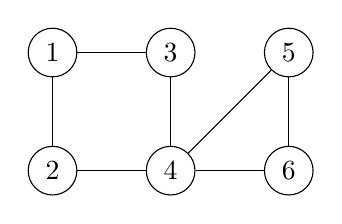
\begin{tikzpicture}[shorten >=1pt,->]
  \tikzstyle{vertex}=[circle, draw]
  \node[vertex] (G_3) at (0,0)   {3};
  \node[vertex] (G_1) at (-1.5,0)  {1};
  \node[vertex] (G_2) at (-1.5,-1.5) {2};
  \node[vertex] (G_4) at (0,-1.5) {4};
  \node[vertex] (G_6) at (1.5,-1.5) {6};
  \node[vertex] (G_5) at (1.5,0) {5};
  
  
  \draw (G_2) -- (G_1) -- cycle;
  \draw (G_1) -- (G_3) -- cycle;
  \draw (G_3) -- (G_4) -- cycle;
  \draw (G_2) -- (G_4) -- cycle;
  \draw (G_5) -- (G_6) -- cycle;
  \draw (G_4) -- (G_5) -- cycle;
  \draw (G_4) -- (G_6) -- cycle;
 
    		\end{tikzpicture}
    		\caption{}
  			\end{subfigure}
  			\hfill
  			\begin{subfigure}[b]{0.45\textwidth}
    		\centering
    		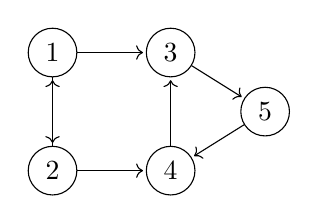
\begin{tikzpicture}[shorten >=1pt,->]
  \tikzstyle{vertex}=[circle, draw]
  \node[vertex] (G_3) at (0,0)   {3};
  \node[vertex] (G_1) at (-1.5,0)  {1};
  \node[vertex] (G_2) at (-1.5,-1.5) {2};
  \node[vertex] (G_4) at (0,-1.5) {4};
  \node[vertex] (G_5) at (1.2,-0.75) {5};
  
  
  \draw (G_2) -- (G_1);
  \draw (G_1) -- (G_2);
  \draw (G_1) -- (G_3);
  \draw (G_4) -- (G_3);
  \draw (G_2) -- (G_4);
  \draw (G_5) -- (G_4);
  \draw (G_3) -- (G_5);
 
    		\end{tikzpicture}
    		\caption{}
  			\end{subfigure}
  \caption{Příklady grafů. (a) Neorientovaný graf. (b) Orientovaný graf.}
  \label{des}
  \end{figure}
  
			Příklady nakreslení grafu vidíme na obrázku \ref{des}.
			Pomocí neorientovaného neohodnoceného grafů můžeme například reprezentovat vztahy mezi lidmi, kde vrcholy budou jednotlivé osoby a hrany povedou mezi těmi dvojicemi vrcholů, které spolu kamarádí. Nebo můžeme pomocí ohodnoceného grafu modelovat síť měst, kde hodnota hran mezi dvěma městy bude značit délku silnice mezi městy. Často se také grafy využívají pro popis \emph{stavového prostoru} her, kde vrcholy představují stavy a hrany mezi nimi akce, kterými lze přejít z jednoho stavu do druhého.
			
			
			\subsection{Reprezentace grafu v počítači}
Existuje několik způsobů, jak efektivně reprezentovat graf v počítači. %Každá metoda má své výhody a nevýhody, a volba závisí na konkrétních potřebách a vlastnostech grafu. 
Uvedu zde dvě nejběžnější metody použitelné pro jak neorientované, tak orientované grafy. Budou určené pro neohodnocené grafy, ale s mírnými úpravami se dají použít i pro ohodnocené grafy.

\begin{itemize}
	\item \emph{Matice sousednosti:} Očíslujeme všechny vrcholy grafu od 1 do $|V|$. Matice sousednosi $A$ má velikost $|V| \times |V|$ a je definovaná jako $A = (a_{ij})$, kde
	
    $$a_{ij}=
    \begin{cases}
      1 & \text{pokud}\ (i,j)\in E, \\
      0 & \text{jinak}.
    \end{cases}$$
  Výhodou této reprezentace je, že zjistit zda jsou dva vrcholy spojené hranou zvládneme v konstantním čase $\mathcal{O}(1)$, vůbec nezáleží na velikosti grafu. Vyjmenování všech následníků vrcholu zabere $\Theta(|V|)$. Nevýhodou je, že zabírá prostor $\Theta(|V|^2)$.
%Pro neorientované grafy je matice symetrická podle hlavní diagonály.
	
	\item \emph{Seznam sousedů:} Vrcholy opět očíslujeme od 1 do $|V|$. Tato reprezentace uchovává pole, které má na $i$-té pozici ukazatel na seznam následníků vrcholu $i$. %$v \in V$ seznam jeho následníků. 
	Tato metoda je efektivnější pro \emph{řídké grafy}, ve kterých $|E| \ll |V|^2$. Zabírá prostor $\Theta(|E|+|V|)$, ale ověřit existenci hrany $(i,j)$ zabere $\mathcal{O}(|V|)$. Výhodou je, že najít všechny následníky vrcholu je lineární s jejich počtem, tedy $\mathcal{O}(\textrm{počet následníků})$.%$\mathcal{O}(\textrm{počet následníků})$
	

\end{itemize}

%Výběr konkrétní reprezentace závisí na konkrétních požadavcích a prováděných operacích nad grafem. Každá metoda má své vlastní využití a přináší efektivitu při určitých typech algoritmů a operací nad grafy.


			\section{Prohledávání do hloubky}
			Algoritmus prohledávání do hloubky (anglicky \emph{depth-first search}, zkráceně \emph{DFS}) je algoritmus pro procházení grafu. Jak implikuje název, DFS prochází graf vždy tak \emph{hluboko}, jak to jde. DFS začne v počátečním vrcholu $v_0$ a prozkoumává vždy hrany naposledy nalezeného vrcholu $v$, z kterého ještě vedou neprozkoumané hrany. Jakmile narazí na takový vrchol, který nemá žádné neprozkoumané sousedy, nemůže už jít hlouběji a metodou nazývanou \emph{backtracking} se vrátí na poslední vrchol s alespoň jedním neprozkoumaným sousedem. Tento proces se opakuje do té doby, než jsou nalezeny všechny vrcholy dosažitelné z $v_0$.

Pro implementaci algoritmu DFS se využívá datové struktury\footnote{Datová struktura je abstraktní způsob ukládání dat v počítači, s kterými umí provádět určité operace.} \emph{zásobník}, případně lze použít namísto zásobníku techniku \emph{rekurze}, která stejně využívá systémový zásobník. Zásobník je datová struktura, která si pamatuje pořadí svých prvků, a řídí se pravidlem LIFO - Last In, First Out%(doslova "poslední přidaný, první odebraný")
. To znamená, že nové prvky přidává na konec a odebírá je rovněž z konce\footnote{Stejně, jako kdybychom chtěli přidat/odebrat náboj ze zásobníku pistole.}. Těmto operacím se obvykle říká PUSH a POP.

DFS se zásobníkem je popsáno pseudokódem \ref{dfs}.
\begin{algorithm}

			    \caption{Prohledávání do hloubky}
			    \label{dfs}
  				\Vst{Graf $G = (V,E)$, počáteční vrchol $v_0 \in V$}
  				Přidej $v_0$ do zásobníku $Z$ a označ $v_0$ jako navštívený.
  				
  				\While{zásobník Z není prázdný}{
				$v \gets$ Z.POP() \Komentar*{Odebere ze zásobníku horní prvek a uloží ho do $v$}
				\For{ všechny sousedy $w$ vrcholu $v$}{
				\If{$w$ není navštívený}{
				Z.PUSH($w$)
				
				Označ $w$ jako navštívený.
				} 
								
				}
  				}
				%$a\gets x, b\gets y$\;  				
  				%\While{můžeš}{
    			%\If{$a < b$}{prohoď $a$ s $b$}
  				%\If{$b = 0$}{vyskoč z cyklu}
  				%$a \gets a \text{ mod } b$ \Komentar*{mod značí zbytek po vydělení $a$ hodnotou $b$}
  				%}
				
				
				\end{algorithm}
\begin{figure}[h]
\begin{center}
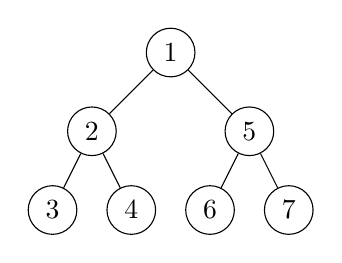
\begin{tikzpicture}[shorten >=1pt,->]
  \tikzstyle{vertex}=[circle, draw]
  \node[vertex] (G_1) at (0,0)   {1};
  \node[vertex] (G_3) at (-1.5,-2)  {3};
  \node[vertex] (G_2) at (-1,-1) {2};
  \node[vertex] (G_4) at (-0.5,-2) {4};
  \node[vertex] (G_5) at (1,-1) {5};
  \node[vertex] (G_6) at (0.5,-2) {6};
  \node[vertex] (G_7) at (1.5,-2) {7};
  \draw (G_1) -- (G_2) -- (G_3) -- cycle;
  \draw (G_1) -- (G_5) -- cycle;
  \draw (G_2) -- (G_4) -- cycle;
  \draw (G_5) -- (G_7) -- cycle;
  \draw (G_5) -- (G_6) -- cycle;
\end{tikzpicture}
\caption{Graf s vrcholy označenými podle pořadí, v jakém je projde DFS} \label{grafDFS}
\end{center}
\end{figure}
			Algoritmus \ref{dfs} pouze navštíví každý vrchol dosažitelný z $v_0$ a označí ho za navštívený, nic ale nevrací. To proto, že DFS je algoritmus na procházení grafu. Mohli bychom ho ale lehce modifikovat tak, aby našel cestu z vrcholu $v_0$ do $v_1$. Konkrétně by si pro každý vrchol pamatoval jeho předchůdce a jakmile by našel cílový vrchol, tak by postupně vypsal cíl, předchůdce cíle, atd. Nevýhodou prohledávání do hloubky je, že pokud ho využijeme k nalezení cesty mezi dvěma vrcholy, nalezená cesta není nutně nejkratší možná, v důsledku pořadí, v jakém DFS prochází vrcholy.
			
			 %	DFS lze využít například pro hledání \emph{komponent souvisloti} grafu.
			
			
			Časová komplexita je $\mathcal{O}(|V| + |E|)$, protože v nejhorším případě projde celý graf. Prostorová složitost je $\Theta(|V| + |E|)$. TODO(zkontrolovat)
			
			\section{Prohledávání do šířky}
			Algoritmus prohledávání do šířky (anglicky \emph{breadth-first search}, zkráceně \emph{BFS}) je dalším algoritmem pro procházení grafu. BFS prochazí graf do \emph{šířky}, tj. postupně prozkoumává všechny sousedy počátečního vrcholu $v_0$, pak sousedy sousedy sousedů  atd. %dříve, než se pohne dál do hloubky.

%Podobně jako u DFS začínáme v počátečním vrcholu $v_0$.
Na rozdíl od DFS používá BFS frontu namísto zásobníku. Fronta je datová struktura, která pracuje podle pravidla FIFO (First In, First Out), což znamená, že prvek, který je v frontě nejdéle, bude odebrán jako první. Operaci přidání prvku na konec fronty se obvykle říká ENQUEUE a odebrání prvku ze začátku fronty DEQUEUE.

Algoritmu se někdy přezdívá "algoritmus vlny", protože nalezne nejdřív všechny vrcholy vzdálené od $v_0$ o jedna (sousedy $v_0$), pak ty vzdálené o dva (sousedy sousedů $v_0$) a tak dále, jako by se z $v_0$ šířila vlna po vodní hladině.

Detailní popis nalezneme v pseudokódu \ref{bfs}.



\begin{algorithm}

			    \caption{Prohledávání do šířky}
			    \label{bfs}
  				\Vst{Graf $G = (V,E)$, počáteční vrchol $v_0 \in V$}
  				Přidej $v_0$ do fronty $Q$ a označ $v_0$ jako navštívený.
  				
  				\While{fronta Q není prázdná}{
				$v \gets$ Q.DEQUEUE() %\Komentar*{Odebere z fronty první pra uloží ho do $v$}
				
				\For{ všechny sousedy $w$ vrcholu $v$}{
				\If{$w$ není navštívený}{
				Q.ENQUEUE($w$)
				
				Označ $w$ jako navštívený.
				} 
								
				}
  				}
				%$a\gets x, b\gets y$\;  				
  				%\While{můžeš}{
    			%\If{$a < b$}{prohoď $a$ s $b$}
  				%\If{$b = 0$}{vyskoč z cyklu}
  				%$a \gets a \text{ mod } b$ \Komentar*{mod značí zbytek po vydělení $a$ hodnotou $b$}
  				%}
				
				
				\end{algorithm}


\begin{figure}[h]
\begin{center}
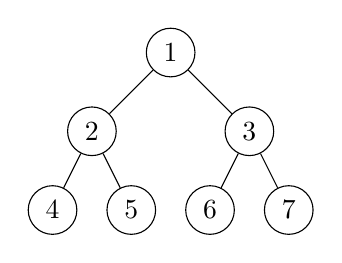
\begin{tikzpicture}[shorten >=1pt,->]
  \tikzstyle{vertex}=[circle, draw]
  \node[vertex] (G_1) at (0,0)   {1};
  \node[vertex] (G_3) at (-1.5,-2)  {4};
  \node[vertex] (G_2) at (-1,-1) {2};
  \node[vertex] (G_4) at (-0.5,-2) {5};
  \node[vertex] (G_5) at (1,-1) {3};
  \node[vertex] (G_6) at (0.5,-2) {6};
  \node[vertex] (G_7) at (1.5,-2) {7};
  \draw (G_1) -- (G_2) -- (G_3) -- cycle;
  \draw (G_1) -- (G_5) -- cycle;
  \draw (G_2) -- (G_4) -- cycle;
  \draw (G_5) -- (G_7) -- cycle;
  \draw (G_5) -- (G_6) -- cycle;
\end{tikzpicture}
\caption{Graf s vrcholy označenými podle pořadí, v jakém je projde BFS} \label{grafBFS}
\end{center}
\end{figure}
Časová složitost BFS je $\mathcal{O}(|V| + |E|)$, což znamená, že v nejhorším případě projde celý graf. Prostorová složitost je $\mathcal{O}(|V| + |E|)$.

Výhodou BFS je to, že při hledání cesty vždy najde nejkratší\footnote{Takovou, která obsahuje nejméně vrcholů.} cestu mezi dvěma vrcholy, případně pozná, že mezi nimi neexistuje cesta. Protože nijak nezapočítává ohodnocení hran, bude i v ohodnocených grafech nacházet cestu s nejméně vrcholy. V takových grafech ale jako nejkratší cestu obvykle považujeme tu, která má nejmenší součet ohodnocení všech hran. Z tohoto důvodu nenalezne BFS optimální cestu na ohodnocených grafech.

%což ho činí vhodným pro hledání nejkratších cest v neohodnocených grafech.
		
			\section{Uspořádané vyhledávání}
			Dosud představené algoritmy jsou primárně určené pro procházení grafů, přestože se dají aplikovat na hledání cesty mezi dvěma vrcholy.
			%, už vůbec nemají žádnou informaci navíc o hledaném vrcholu. 
			Naopak další algoritmy, které představím, jsou zaměřené na hledání optimálních cest, a to i v ohodnocených grafech.
			
			%a jsou \emph{informované}, což znamená, že mají navíc informaci o odhadu vzdálenosti každého vrcholu $v \in V$ od cílového vrcholu. Princip těchto algortimů pochází z intuitivní myšlenky, že pokud budeme hledat nejkratší cestu z Prahy do Brna, nebudeme jako první zvažovat cestu procházející Plzní a podobně.  
			
			%Tento odhad pro každý vrchol typicky zprostředkovává nějaká \emph{heuristická funkce $h(n)$}. 
			
			Tyto algoritmy vybírají který vrchol \emph{expandovat}\footnote{Expanzí vrcholu myslíme jeho prozkoumání a přidání jeho neprozkoumaných sousedů do fronty.} jako další v pořadí podle nějaké evaluační funkce $f : V \rightarrow \mathbb{R}$. Ta vrací nějakou reálnou hodnotu pro každý vrchol $v \in V$. 
			Hromadně se označují jako algoritmy třídy uspořádaného vyhledávání (anglicky best-first search), protože pořadí, v jakém prohledávají vrcholy, je nějak uspořádané podle $f$.

			Typicky se jako první prochází vrchol $v$ s nejmenší hodnotou $f(v)$. K tomu se často používá prioritní fronta, která řadí své prvky vzestupně podle priority, přiřazené ke každému prvku. Většinou se implementuje pomocí datové struktury \emph{haldy}. Více o haldách viz \cite{pruvodce}.			
			
			Poznámka: při rešerši na uspořádané vyhledávání jsem se častokrát setkával s rozlišnou terminologií. V některých zdrojích \cite{carlos} se jako best first-search označuje algoritmus, který jiní \cite{patel_intro} pojmenovávají jako greedy best-first search. Jiní \cite{uhlik,wiki_best_first,felner} zase považují best-first search jako algoritmický princip nebo třídu algoritmů.
			 %podobně v českých zdrojích se někdy uspořádaným vyhledáváním myslí třída algoritmů, někdy samotné hladové uspořádané vyhledávání. 
			 Já jsem zvolil stejné pojmenování jako \cite{patel_intro, uhlik, felner}, protože mi přišlo nejvíce konzistentní a logické.
			%určují, v jakém pořadí procházet vrcholy, se označují jako algoritmy třídy uspořádaného vyhledávání. 
			
			
			
			%tzn. rozhodují se, v jakém pořadí prozkoumávat vrcholy na základě nějaké funkce $f(v)$. 

			\subsection{Uniform Cost Search}
			Uniform cost search, dále jen UCS, je algoritmus třídy uspořádaného vyhledávání, který najde optimální %nejlevnější\footnote{Jako nejlevnější cestu označujeme cestu s nejnižším součtem vah všech hran cesty.} 
			cestu mezi počátečním vrcholem $v_0$ a cílovým vrcholem $c$ v grafu s kladně ohodnocenými hranami. 
			UCS funguje podobně jako BFS, jen místo postupného prohledávání vrcholů ve stejné hloubce (se stejným minimálním počtem hran od startu) prohledává UCS ve "vrstvách" stejné ceny.
			
			%UCS funguje velmi podobně jako BFS, jen se místo hladin vrcholů stejně vzdálených od $s$ uvažuje vrcholy se stejným $g(v)$.
			Evaluační funkcí pro UCS je $f(v) = g(v)$, kde $g(v)$ je cena cesty mezi počátečním vrcholem $s$ a vrcholem $v$. 
			UCS používá prioritní frontu, většinou označovanou jako OPEN. Na začátku je do ní vložen pouze počáteční vrchol s prioritou 0. V každé iteraci je z OPEN odebrán vrchol s největší prioritou a expandován. Největší prioritu mají prvky s nejnižší $g(v)$. To znamená, že UCS vždy expanduje vrchol s nejnižší kumulativní cenou od počátečního vrcholu $s$ a tudíž nalezne optimální cestu do každého vrcholu, protože jinak by už byl vrchol expandovaný po levnější cestě. Expandované vrcholy jsou přidané do seznamu CLOSED. Pro následníky expandovaného vrcholu $v$, kteří nejsou v CLOSED, je spočítaná jejich $g$ hodnota pro cestu z vrcholu $s$ přes $v$. V případě, že ještě nejsou v OPEN, jsou tam přidané s vypočtenou prioritou. V opačném případě už v OPEN jsou s nějakou $g$ hodnotou, pak pouze pokud je nová $g$ hodnota menší než předešlá $g$ hodnota, je jejich priorita v OPEN aktualizována.
			
			 V průběhu běhu algoritmu si budeme pro každý expandovaný vrchol označovat jeho předchůdce. Díky tomu můžeme po nalezení cílového vrcholu rekonstruovat cestu vedoucí z $v_0$ do $c$.
			
			
			
			%UCS funguje stejně jako Dijkstrův algoritmus, s tím rozdílem že Dijkstrův algoritmus tak, jak je klasicky popisován, zařadí na začátku do prioritní fronty všechny vrcholy s cenou $\infty$, až na $s$, který má cenu $0$.
			Podbrobně popsaný je UCS v pseudokódu \ref{ucs}.
			

			\begin{algorithm}[H]

			    \caption{Uniform cost search}
			    \label{ucs}
  				\Vst{Graf $G = (V,E)$, počáteční vrchol $v_0 \in V$, hledaný vrchol $c \in V$}
  				\Vyst{Seznam $rodice$, uchovávající předchůdce každého nalezeného vrcholu, $g$ uchovávající cenu cesty do každého nalezeného  vrcholu; nebo informaci o neúspěchu}
  				%Přidej $v_0$ do $OPEN$ \\% a označ $v_0$ jako navštívený.
  				$g(v_0) \gets 0$ \Komentar*{$g(n)$ je cena cesty z $v_0$ do $n$}
  				Vlož $v_0$ do $OPEN$\\
  				
  				$CLOSE \gets \emptyset$ \Komentar*{$CLOSE$ je prázdný seznam}
  				$rodice(v_0) \gets \emptyset$\\ %\Komentar*{$rodice(v)$ obsahuje předchůdce $v$, skrz kterého vede nejkratší cesta do $v$}
  				%$cena(v_0) \gets 0 $
  				
  				\While{OPEN není prázdný}{
				$u \gets$ OPEN.extractMin() \Komentar*{Odebere z fronty vrchol s nejmenší hodnotou $g$ a uloží ho do $u$}
				
				\If{$u$ je $c$}{
				Vrať $rodice, g$ 
				}
				Vlož $u$ do $CLOSED$\\
				\For{všechny následníky $v$ vrcholu $u$, kteří nejsou v CLOSED}
				{
				$tmpG \gets g(u) + w(u,v)$ \Komentar*{$w(u,v)$ je váha							hrany $(u,v)$}
				\If{$v$ není v $OPEN$}{
				$g(v) \gets tmpG$\\
				$rodice(v) \gets u$ \Komentar*{Nastaví vrchol $u$ jako předchůdce $v$}
				Vlož $v$ do $OPEN$
				}
				\ElseIf{$v$ je v $OPEN$ a $tmpG$ je menší než $g(v)$}{
				$g(v) \gets tmpG$\\	
				$rodice(v) \gets u$\\
				}
				}

  				}
  				Vrať $nenalezeno$
		\end{algorithm}
				
				Často se setkáme s podobným algoritmem, nazývaným \emph{Dijkstrův algoritmus}. Ten se od UCS liší minimálně, rozdíly mezi nimi a argumenty pro používaní UCS v praxi jsou popsané v \cite{felner}.
			
			\subsection{Hladové uspořádané vyhledávání}
			Algoritmus hladového uspořádaného vyhledávaní (anglicky greedy best-first search) je dalším algoritmem pro hledání cesty v kladně ohodnoceném grafu. Pracuje na předpokladu, že pokud bude opakovaně \emph{expandovat} vrchol, který je zdánlivě nejblíž k cílí, najde cestu do cíle nejrychleji. Princip tohoto algoritmu pochází z intuitivní myšlenky, že pokud budeme hledat nejkratší cestu z Prahy do Brna, nebudeme jako první zvažovat cestu procházející Plzní a podobně. 
			%Jinak řečeno předpokládá, že nejkratší cesta povede stejným směrem, jakým je cíl. 
			
			Jedná se o \emph{informovaný} algoritmus, což znamená, že má navíc informaci o odhadu vzdálenosti každého vrcholu $v \in V$ od cílového vrcholu. 
			Tento odhad je typicky zprostředkován \emph{heuristickou funkcí $h(v)$}.
			
			%Ideální funkce by pro každý vrchol vrátila jeho skutečnou vzdálenost od hledaného vrcholu, ale takovou funkci obvykle k dispozici nemáme, proto se používají \emph{heuristické funkce}. 
			Heuristické funkce (heuristiky) můžou být jakékoli, pokud např. při hledání cesty mezi dvěma lokacemi budeme znát jejich souřadnice, můžeme je využít pro výpočet heuristiky. %hledáme-li cestu např. mezi městy Evropy nebo na čtverečkovaném papíře s nakreslenými překážkami, často víme o vrcholech grafu, kterým tyto situace reprezetujeme, nejen jejich hrany ale i jejich přesné souřadnice. 

%\subsection{Heuristické funkce}
			Nejčastěji používané heuristické funkce jsou:
			\begin{enumerate}
			
\item \textbf{Eukleidovská vzdálenost:} $h(v) = \sqrt{(x_c - x_v)^2 + (y_c - y_v)^2}$, kde $x_c$,$y_c$ jsou souřadnice cílového vrcholu a $x_v, y_v$ jsou souřadnice vrcholu $v$. Tuto heuristiku lze použít na grafy reprezentující klasické mapy.

\item \textbf{Manhattanská vzdálenost:} $h(v) = |(x_c - x_v)| +
|(y_c - y_v)|$, kde $x_c$,$y_c$ jsou souřadnice cílového vrcholu a $x_v, y_v$ jsou souřadnice vrcholu $v$. Tato heuristika je ideální pro mapy reprezentované čtvercovou mřížkou, kde jsou povoleny pouze vertikální a horizontální pohyby.

\item \textbf{Octile heuristika:} $h(v) = \Delta x+ \Delta y + (\sqrt{2}-2) \cdot min(\Delta x, \Delta y)$, kde $\Delta x = |x_c - x_v|, \Delta y = |y_c - y_v|$ %jsou absolutní rozdíly souřadnic vrcholů, podle souřadnic $x$ a $y$. 
Tato heuristika je ideální pro osmisměrné čtvercové mřížky, tedy takové, kde je kromě vertikálního a horizontálního pohybu povolen i diagonální pohyb. Počítá s cenou 1 pro vertikální a horizontální pohyby a cenou $\sqrt{2}$ pro diagonální.
\end{enumerate}
Heuristická funkce $h(n)$ je \emph{přípustná}, pokud pro každý vrchol $v \in V$ platí $h(v) \leq h^*(v)$, kde $h^*(v)$ je \emph{ideální} heuristika, tedy skutečná vzdálenost od cíle.
%Navíc pokud platí i $TODO$, pak funkci označujeme jako \emph{monotónní}.			
			
			
			Pro hladové uspořádané vyhledávání se evaluační funkce rovná heuristické funkci: $f(v) = h(v)$. 						
			
			Na začátku vloží do prioritní fronty počáteční vrchol s prioritou 0.
			Dokud není prioritní fronta prázdná, tak v každé iteraci vybere z prioritní fronty vrchol s nejmenší $f(v)$ a ten expanduje, dokud nedorazí do cíle.
			
			Nevýhodou tohoto algoritmu je, že vrcholy prozkoumává jen podle heuristiky. %se snaží jít směrem do cíle, i když tím směrem nemusí vést optimální cesta.
			Jeho efektivita záleží na přesnosti heuristické funkce, pokud by byla heuristika ideální prozkoumá jen vrcholy vedoucí do cíle a to po optimální cestě. Jeho ohodnocovací funkce nepřihlíží k vzdálenosti od počátečního vrcholu a algoritmus nijak nezohledňuje celkovou ušlou vzdálenost od počátečního vrcholu, což může vést k nalezení neoptimálních cest. Nicméně nějakou cestu najde většinou rychleji než UCS, protože prozkoumáváním vrcholů zdnálivě bližších k cíli jako první často sníží celkový počet prozkoumaných vrcholů.
			
			
			%Protože jeho ohodnocovací funkce nijak nezohledňuje vzdálenost od počátečního vrcholu a nijak nepracuje s celkovou ušlou vzdáleností od počátečního vrcholu, vede to k nacházení dlouhých neoptimálních cest.
			
			%má za následek, že algoritmus nenajde vždy optimální řešení
		
			Poznámka: algoritmu se říká hladový, protože jako hladové algoritmy se označují ty algoritmy, které v každém kroku volí lokální optimum s vidinou, že tyto volby povedou celkově do globálního optima, neboli k optimálnímu řešení. 			
			%Tímto způsobem se algoritmus velmi agresivně vrhne směrem k cíli, avšak pokud narazí ...dopsat
			
			
			%Toto vede sice rychlému, ale ne vždy optimálnímu hledání. Algoritmus je náchylný k přecenění první cesty, což má za následek nenalezení nejkratší (optimální) cesty.
						
			\subsection{Algoritmus A*}
			Algoritmus A* navrhli Peter Hart, Nils Nilsson a Bertram Raphael v roce 1968. % pro jejich robota. 
			Algoritmus A* kombinuje efektivitu hladového uspořádaného vyhledávání s optimalitou algoritmu UCS.
			
			Tento algoritmus jako svou ohodnocovací funkci $f(v)$ využívá součet heuristické funkce $h(v)$ a funkce $g(v)$, která udává délku nejkratší cesty z počátečního vrcholu do vrcholu $v$: $f(v) = g(v) + h(v)$. 
			
			Protože je to další algoritmus z třídy uspořádaného vyhledávání, funguje podobně jako UCS i hladové uspořádané vyhledávání.
			 A* taktéž prochází vrcholy grafu podle hodnoty ohodnocovací funkce a vybírá vrcholy s nejnižší hodnotou $f(v)$, jediným rozdílem je ohodnocovací funkce samotná.
			%Navíc pokud nalezne pro nějaký vrchol kratší cestu z počátku, updatuje jí. 
			Pokud bude $h(v)$ přípustná, pak A* vždy najde optimální cestu do cílového vrcholu, 
			
			
			Pokud máme takovou heuristiku, že $\forall v \in V:h(v) = 0$ tak A* degraduje do UCS, naopak pokud $\forall v \in V:g(v) = 0 $ tak A* degraduje do hladového uspořádaného vyhledávání.
			
			A* je velmi populární volbou pro implementaci pathfindingu ve hrách nebo v mapových aplikacích pro jeho optimalitu a zároveň efektivitu a rychlost výpočtu. Existují i optimalizované verze A*, které například omezují paměťové nároky.
			
			
			
	
	\part{Implementace vizualizačního programu}
	
		
		
		\chapter{Plánování}
			\section{Představení použitého software}
		
		\chapter{Implementace}
		
		\chapter{Ukázky využití}
		
		\chapter{Výpisy použitých programů}




	\chapter*{Závěr}
	
		Tady bude závěr.
	
	\nocite{*}
    \printbibliography					% Vytvoří seznam literatury
	\addcontentsline{toc}{chapter}{Bibliografie}
    \printglossary[title={Zkratky}]		% Vytvoří seznam zkratek
    \listoffigures						% Vytvoří seznam obrázků
    \listoftables						% Vytvoří seznam tabulek

    \begin{appendices}
	\chapter{Příloha s kódem}	

	\end{appendices}
\end{document}
